\chapter{Background}
\label{chap:background}

This chapter introduces the theoretical background for understanding the idea
behind \texttt{Crotosolve}.
Rather than giving a complete overview of the field, this text is strictly
focused on aspects critical for proving the optimizer's correctness and
understanding its applications.
I will first present an introduction to the theory of quantum information
processing using qubits, gates, and circuits.
Following this introduction, I will also give a quick introduction to the field
of Machine Learning.
I will show how Quantum Machine Learning applies the ideas from Machine Learning
to quantum processing devices.
The final section of this chapter will focus on state-of-the-art classical and
quantum optimization techniques in particular.
One of these optimization methods is \texttt{Rotosolve}, which I will present
with further detail.
These basic ideas are also fundamental for the \texttt{Crotosolve} algorithm,
which will be developed in the next chapter.

\section{A brief introduction to quantum computing}
\label{sec:quantum-intro}
% TODO: Mention that this is an abstract level? quantum hardware implementation
At its core, the operation of a quantum computer revolves around gates and
qubits.
Qubits (quantum bits) make up the data register of a quantum computer.
Just like a classical bit can be in the $0$ or $1$ state, a qubit can be in a
corresponding $\ket 0$ or $\ket 1$ state.
Besides these two basis states, however, quantum bits can be in a superposition
of these two states,

$$\ket \psi = \alpha_0 \cdot \ket 0 + \alpha_1 \cdot \ket 1\,,$$

where the probability amplitudes $\alpha_0, \alpha_1 \in \mathbb C$ can be any
complex numbers with $\left|\alpha_0\right|^2 + \left|\alpha_1\right|^2 = 1$.
The superposable character of a qubit essentially increases its expressibility
in comparison to a classical, digital bit from the discrete set
$\left\{0, 1\right\}$ to the complex, two-dimensional sphere surface
$\left\{\vec \alpha \in \mathbb C^2 \mid \left|\vec\alpha\right|^2\right\}$.
Thus, a quantum computer with a single qubit can work with continuous,
multidimensional data, while a classical computer with a single bit can only
work with a single boolean value.

Due to the laws of quantum mechanics, this multidimensional superposition state
collapses into one of its discrete basis states upon observation.
More specifically, this means that \emph{measuring} the value of a qubit cannot
reveal its probability amplitudes and instead turns the state into either
$\ket 0$ (i.e., $\alpha_0 = 1, \alpha_1 = 0$) or
$\ket 1$ (i.e., $\alpha_0 = 0, \alpha_1 = 1$)\footnote{
    Technically, it is possible to measure the state in a different basis, like
    $\ket + = \frac{\ket 0 + \ket 1}{\sqrt 2}$ and
    $\ket - = \frac{\ket 0 - \ket 1}{\sqrt 2}$.
    However, this will not be necessary for the development of
    \texttt{Crotosolve}.
}.
The probability of the qubit collapsing into either of these states is given by
the squared absolute value of its probability amplitude,

$$\mathbb P(M = \ket n) = \left| \alpha_n \right|^2,\, n \in \left\{0, 1\right\}.$$

Thus, the normalization of the probability amplitudes, 
$\sum_{n \in \left\{0, 1\right\}} \left|\alpha_n\right|^2 = 1$, is in fact a
normalization of the probability distribution over the given basis states.
While it is physically impossible to observe $\alpha_0$ and $\alpha_1$ directly,
their squared absolute values still influence the outcome of observation $M$.
If the same\footnote{
    Two quantum states $\sum \alpha_n \ket n$ and $\sum \beta_n \ket n$ are the
    same if all of their probability amplitudes are the same,
    i.e., $\alpha_n = \beta_n \forall n$.
} quantum state can be prepared many times, $\left|\alpha_n\right|^2$ can be
estimated as the relative frequency from an empirical probability distribution
of $M$.

Since only the absolute value of $\alpha_0$ and $\alpha_1$ influences the
measurement outcome, it is common to rewrite the state as follows.

\begin{equation}
    \begin{split}
        \ket \psi
            &= \alpha_0 \ket 0 + \alpha_1 \ket 1\\
            &= e^{i\gamma} \left(\cos \frac\theta2 \ket 0 + e^{i\varphi} \sin \frac\theta2 \ket 1\right)
    \end{split}
\end{equation}

\begin{figure}
    \centering
    \begin{blochsphere}[radius=3 cm,tilt=15,rotation=-20,opacity=0]
        \drawBallGrid[style={opacity=0.1}]{30}{30}

        \drawAxis[]{0}{0} % Z axis
        \labelLatLon{up}{90}{0};
        \labelLatLon{down}{-90}{90};
        \node[above] at (up) {{$\left|0\right>$ }};
        \node[below] at (down) {{$\left|1\right>$}};

        \drawAxis[]{90}{0} % Y axis
        \labelLatLon{right}{0}{0};
        \labelLatLon{left}{0}{180};
        \node[right] at (right) {{$\left|R\right>$ }};
        \node[left] at (left) {{$\left|L\right>$}};

        \drawAxis[]{90}{90} % X axis
        \labelLatLon{front}{0}{90};
        \labelLatLon{back}{0}{-90};
        \node[below] at (front) {{$\left|+\right>$ }};
        \node[above] at (back) {{$\left|-\right>$}};
    \end{blochsphere}
    \caption{The Bloch sphere can represent the state
        $\ket\psi = e^{i\gamma} \left(\cos \frac\theta2 \ket 0 + e^{i\varphi} \sin \frac\theta2 \ket 1\right)$
        of a single qubit, ignoring its global phase.
        $\varphi$ specifies the rotation of the state around the $Z$ axis
        ($\ket 0 \to \ket 1$).
        $\theta$ specifies the rotation of the state relative to the $XY$ plane
        ($X$ axis: $\ket - \to \ket +$, $Y$ axis: $\ket L \to \ket R$).}
    \label{fig:blochsphere}
\end{figure}

In this representation, $e^{i\gamma}$ has no effect on the outcome of
measurement $M$ because $\left|e^{i\gamma}\right| = 1$.
That is why the \emph{global phase} $\gamma$ is often ignored.
The remaining two variables $\theta$ and $\varphi$ can be interpreted as
coordinates on the so-called Bloch sphere, which is shown in
\autoref{fig:blochsphere}.

\subsection{Multi-qubit-systems}
The separated state of several qubits can be combined into a multi-qubit state
through the Kronecker product.
With two qubits, this results in

\begin{equation}
    \label{eq:separate-state}
    \begin{split}
        &\left(\alpha_0 \ket 0 + \alpha_1 \ket 1\right) \otimes \left(\beta_0 \ket 0 + \beta_1 \ket 1\right) \\
        = &\alpha_0\beta_0 \ket 0 \otimes \ket 0 + \alpha_0\beta_1 \ket 0 \otimes \ket 1 + \alpha_1\beta_0 \ket 1 \otimes \ket 0 + \alpha_1\beta_1 \ket 1 \otimes \ket 1 \\
        = &\underbrace{\alpha_0\beta_0}_{=: \gamma_{00}} \ket{00} + \underbrace{\alpha_0\beta_1}_{=: \gamma_{01}} \ket{01} + \underbrace{\alpha_1\beta_0}_{=: \gamma_{10}} \ket{10} + \underbrace{\alpha_1\beta_1}_{=: \gamma_{11}} \ket{11}.
    \end{split}
\end{equation}

with $\sum_{n \in \left\{00, 01, 10, 11\right\}} \left|\gamma_n\right|^2 = 1$.
I use natural numbers instead of bitstrings to simplify the notation in the
following.
For example, \autoref{eq:separate-state} can be compactly rewritten to the
following.

\begin{equation}
    \label{eq:separate-state-natural-numbers}
    \begin{gathered}
            \gamma_{00} \ket{00} + \gamma_{01} \ket{01} + \gamma_{10} \ket{10} + \gamma_{11} \ket{11}\\
        =   \gamma_0 \ket 0 + \gamma_1 \ket 1 + \gamma_2 \ket 2 + \gamma_3 \ket 3\\
        =   \sum_{j=0}^3 \gamma_j \ket j
    \end{gathered}
\end{equation}

Similarly to this two-qubit example, a system with $n$ separate qubit states
$\ket{\psi_i}, 1 \leq i \leq n$ can be described with a product state.
In this system, the probability amplitudes
$\gamma_0, \dots, \gamma_{2^n -1} \in \mathbb C$ of the standard basis states
$\ket 0, \dots, \ket{2^n -1}$ are again given by the multiplication and form a
probability distribution through their squared absolute values.

\begin{equation}
    \label{eq:separate-state-n}
    \ket\psi = \bigotimes_{i=1}^n \ket{\psi_i} = \sum_{j=0}^{2^n -1} \gamma_j \ket j
        \quad\text{with}\quad \sum_{j=0}^{2^n -1} \left|\gamma_j\right|^2 = 1
\end{equation}

\subsection{Gates and circuits}

Unlike with classical bits and gates, it is physically impossible for a quantum
computer to create copies of a qubit.
While classical computers typically read (i.e., copy), transform (e.g., add two
numbers), and write data from and to registers, quantum computers can only
perform in-place operations.

Quantum states can be changed by applying operators to them.
Since the state of an $n$-qubit-system can be described through its probability
amplitudes $\gamma_i$, we can represent this state with a $2^n$-dimensional
complex vector.
If we identify $\ket 0 \equiv \begin{pmatrix}1 & 0\end{pmatrix}^\top$ and
$\ket 1 \equiv \begin{pmatrix}0 & 1\end{pmatrix}^\top$,
equation \ref{eq:separate-state-n} implicitly leaves us with

\begin{equation}
    \ket\psi \equiv \begin{pmatrix} \gamma_{0^n} \\ \vdots \\ \gamma_{1^n}\end{pmatrix}\,.
\end{equation}

Universal quantum computers allow us to apply operations to these states that
are described by unitary matrices\footnote{
    A matrix $A \in \mathbb{C}^{N \times N}$ is called unitary if and only if
    its conjugate transpose is its inverse, i.e. $\overline{A^\top} = A^{-1}$.
}.
% COMMONLY USED EXAMPLE GATES, PARAMETERIZABLE (CONTROLLED) ROTATIONAL PAULI
%  GATES IN PARTICULAR
% UNIVERSAL GATE SETS
% TODO: MEASUREMENTS
Such an operation is referred to as a \emph{gate} in quantum computing.
Gates can act on one or multiple qubits, and bigger gates can be composed by
computing the Kronecker product of gates.

The application of gates to a system of qubits can be visualized through
quantum circuits.
In these circuits, each qubit is displayed as a horizontal line, and gates are
displayed as boxes that overlay the lines of the qubits they are applied to.
Measurements are indicated by a box with a meter inside.

Take for example the Hadamard gate $H$,

\begin{equation}
    H = \frac{1}{\sqrt 2}\begin{pmatrix}1 & 1 \\1 & -1\end{pmatrix}\,.    
\end{equation}

\begin{figure}[]
    \centering
    \begin{quantikz}
        \lstick{\ket{0}}    & \gate{H}  & \meter\qw
    \end{quantikz}
    \caption{
        In this single-qubit quantum circuit, a Hadamard gate is applied to the
        qubit before it is measured.
        This circuit will probabilistically output $\ket 0$ just as often as
        $\ket 1$.
    }
    \label{fig:H-circuit}
\end{figure}

Applying the Hadamard gate to a single qubit will transform the
$\ket 0$ state into $\frac{1}{\sqrt 2}\ket 0 + \frac{1}{\sqrt 2}\ket 1$ and
$\ket 1$ into $\frac{1}{\sqrt 2}\ket 0 - \frac{1}{\sqrt 2}\ket 1$, which are
both equal superpositions of the original states.
\autoref{fig:H-circuit} visualizes the application of a Hadamard gate in a
quantum circuit.

All single-qubit gates $U \in \mathbb{C}^{2 \times 2}$ can be represented by
products of \emph{rotational Pauli gates} $RX(\theta), RY(\theta)$ and
$RZ(\theta)$,

\begin{equation}
    \label{eq:rotational-pauli-gates}
    RP\left(\theta\right) = \cos\left(\frac\theta2\right) \cdot I_2 - i \cdot \sin\left(\frac\theta2\right) \cdot P,\quad
    P \in \left\{X, Y, Z\right\}
\end{equation}

These gates are called \emph{parameterized gates} since they can be adjusted by a
continuous parameter $\varphi \in \left[0, 2\pi\right]$.
The Hadamard gate, for example, can be written as
$H = RX(\pi) \cdot RY(0.5\pi)$.

Single-qubit operations can be simulated trivially by computing the product of
the gate matrices and the state vector.

The problem gets more interesting with two-qubit gates.
For example, the controlled $X$ gate (also known as $CNOT$) works on a system
of two qubits and maps the basis states as follows:

\begin{gather}
    \label{eq:cx-zbasis}
    CX = \begin{pmatrix}
        1&0&0&0\\
        0&1&0&0\\
        0&0&0&1\\
        0&0&1&0
    \end{pmatrix}\\
    CX \ket{00} = \ket{00}\\
    CX \ket{01} = \ket{01}\\
    CX \ket{10} = \ket{11}\\
    CX \ket{11} = \ket{10}
\end{gather}

When applying the $CX$ gate to states from the computational basis, the second
bit is flipped ($X$ is applied) if and only if the first bit is $\ket 1$.
States other than those from the computational basis might, however, not follow
this simple principle.
The $\ket{++}$ state, for example, is transformed into the
$\ket{-+} = CX \ket{++}$ state, changing the control qubit but not the target
qubit.

% TODO: Rotation and controlled rotation gates

\section{Quantum Machine Learning}
\label{sec:qml-intro}

Today's quantum devices are far from ideal implementations of the qubits, gates,
and circuits presented in \autoref{sec:quantum-intro}.
Noise is a major limitation of today's quantum devices.
Noise is hard to describe completely since it can be the result of a multitude
of factors.
For example, noise can be accumulated over time by unwanted interactions of the
physical qubit implementation with the outside world.
Additionally, the number of qubits on today's quantum devices is limited to a
couple dozen or a couple hundred.
On quantum computers with high numbers of qubits, the connection topology is
incomplete, as this simplifies the architecture of the physical system. 
This means that multi-qubit gates cannot be applied to arbitrary groups of
qubits directly.
This limitation can be mitigated through the application of swap gates prior
to the multi-qubit gate application, however, this further increases the quantum
computer's exposure to noise.
The limitations of today's quantum devices are collectively referred to as the
\emph{noisy intermediate-scale quantum} (NISQ) era
\cite{preskill_quantum_2018,nielsen_quantum_2007}.
% TODO: maybe move to QC chapter?

Research suggests that Quantum Machine Learning and Variational Quantum
Algorithms may produce useful results even in the presence of NISQ limitations
\cite{cerezo_variational_2021}.
In the following section, I will first introduce a few ideas from classical
Machine Learning.
Using these results, I will present several approaches to Quantum Machine
Learning.
I will focus on optimization techniques in particular, as from Chapter
\ref{chap:gradient-free} onwards, I will introduce a new optimizer that can
produce results in this regime with high efficiency.

\subsection{Classical Machine Learning}
\label{sec:classical-ml-intro}

\begin{figure}
    \centering
    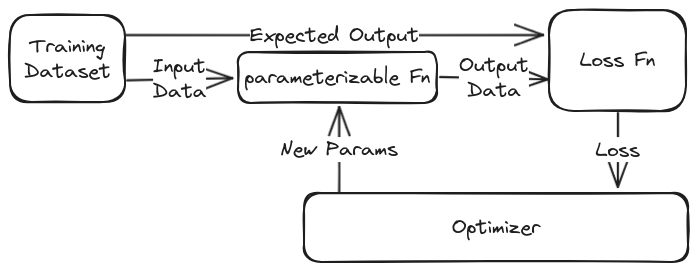
\includegraphics[width=0.8\textwidth]{ml-training-loop}
    \caption{In a typical supervised Machine Learning optimization loop, the
        optimizer runs the model with training data to compute a loss value.
        It updates the model's parameters to reduce the loss value in the next
        evaluation.
        Through many iterations of this process, the model learns the relation
        between input and output data \cite{bishop_pattern_2006}.}
    \label{fig:ml-training-loop}
\end{figure}

According to Bishop \cite{bishop_pattern_2006}, Machine Learning typically aims
to find and reproduce a pattern in a dataset.
In a \emph{supervised} Machine Learning task, a set of input data is given
together with its corresponding output data.
This data could, for example, be the results of an experiment where the input
represents the parameters of the experiment and the output represents the
measurement results corresponding to these parameters.
The goal of a supervised Machine Learning task is to recognize the relation
between input and output data to predict output values from input values.
We measure the quality of the Machine Learning results with a
\emph{loss value}, which is a real number representing how much the predicted
values deviate from the correct values from the output data set.
% TODO: we!

Many approaches in Machine Learning use a parameterizable \emph{model} function
to express the mapping from input to output.
An \emph{optimizer} feeds data into the model and compares the model's
prediction with the correct output to determine the loss value.
Based on this loss value, it updates the parameters of the model aiming to
produce a better loss value in the next model evaluation. 
The repeated process of evaluating test data with the model and updating the
model's parameters based on the generated loss value is often referred to as the
\emph{optimization loop}.
The optimization loop of a supervised Machine Learning process is visualized in
\autoref{fig:ml-training-loop}.
% TODO: model selection, example NN.
% TODO: learning
% TODO: generalization

It should be noted that supervised learning is not the only type of
Machine Learning task.
\emph{Unsupervised} learning tasks, for example, can be implemented without
given output data.
In this case, the loss value must be determined from the model output without
relying on any given ideal output data.
When applying Machine Learning to an optimization problem, the loss value is
typically the negative objective value of the output proposed by the model
function.

The success of a Machine Learning task depends on the careful selection of
training data, loss function, model, and the optimizer.
For the optimizer, a common choice is \emph{Gradient Descent}.
In each optimization iteration, the optimizer computes the gradient of the loss
value from the model output w.r.t. the model parameters.
As the gradient points towards the steepest ascent, its negative points towards
the steepest descent.
Altering the parameters in this direction should then decrease the loss value.
This parameter update can be expressed with the following equation, where
$\mathbf{\theta}_i$ is the parameter vector after the $i$-th iteration, $E$ is
the loss function, $f$ is the model, $(x,y)$ is the training data, and $\eta$ is
the learning rate.

\begin{equation}
    \mathbf{\theta}_{i+1} = \mathbf{\theta}_i - \eta\nabla E(f_{\mathbf{\theta}_i}(x), y)
\end{equation}

% TODO: explain learning rate and adam
% TODO: mention adam and adagrad as two improvements

\subsection{Quantum Machine Learning}
\label{sec:real-qml-intro}
% TODO: rename, sec and subsec have the same name

As Machine Learning can often learn patterns from given datasets even in the
presence of noise, it is expected that Machine Learning applications can benefit
from the computational power of quantum computers even in the NISQ era
\cite{ciliberto_quantum_2018,cerezo_variational_2021}.

One approach for using quantum computers for Machine Learning is to use
PQCs as the model function of an otherwise classical optimization loop.
This is referred to as a \emph{hybrid} approach
\cite{benedetti_parameterized_2019,mitarai_quantum_2018}.

% TODO: cite schuld review?
% TODO: parameter shift rule (schuld, mitarai)
% TODO: VQE as an example
% TODO: maybe QNG?

\subsection{Optimization techniques}
\label{sec:optimizers}

Although gradient-based optimizers are widely used in the field of Machine
Learning, other optimizers are available too.
For the optimization of PQCs, Ostaszewski et al. present an alternative approach
that optimizes model parameters independently \cite{ostaszewski_structure_2021}.
In ``\emph{\citefield{ostaszewski_structure_2021}{title}}'', they observe that
the expected loss value $\mathbb P(M = \ket 0)$ of a PQC w.r.t. a single
rotational Pauli gate parameter $\theta$ always has the following mathematical
structure.

\begin{equation}
    \mathbb{P}(M = \ket 0 | \theta) = d_1 + d_3 \cdot \cos(\theta + d_2)
\end{equation}

Here, $d_1, d_2, d_3 \in \mathbb R$ are unknown constants independent of $\theta$.
The authors could reconstruct these constants by evaluating the PQC with three
select values for $\theta$.
As sinusoidal functions are well understood, the minimum of this reconstructed
function can be calculated analytically.
It is mathematically easy to
calculate their minimum once the function is reconstructed.
